\documentclass[conference]{IEEEtran}

\usepackage[dvips]{graphicx}
%\usepackage{graphicx}
\usepackage{amsmath,amssymb}
\usepackage{algorithm}
\usepackage{algorithmic}
\usepackage{subcaption}

\begin{document}
\title{To Be Done}
%\title{Paper Title (Each Word of the Title Should Begin with a Capital Letter with the Exception of Articles and Conjunctions)}
\date{}%date stay empty

\author{
\IEEEauthorblockN{Luca Comanducci, Michele Buccoli,\\ Massimiliano Zanoni, Augusto Sarti}
\IEEEauthorblockA{Line 2 - Name of organization1 \\ Line 3 - City1, Country1 \\ Line 4 - {Author1, Author2}@domain.edu\\}
\and
\IEEEauthorblockN{Stefano Delle Monache\\ }
\IEEEauthorblockA{Name of organization2 \\ City2, Country2 \\ Author3@domain.edu\\}
\and
\IEEEauthorblockN{Giovanni Cospito}
\IEEEauthorblockA{Name of organization2 \\ City2, Country2 \\ Author3@domain.edu\\}}


\maketitle


\begin{abstract}
The abstract describes a summary of the paper. In some cases, the authors confuse the abstract with the introduction. In the abstract using of acronyms and abbreviations is undesirable.  
\end{abstract}

\section{Introduction}\label{sec:introduction}
With the rapid evolution of technology and the increase speed of network connections, numerous applications have become possible.  

Computer-aided musical collaborations between geogra\-phically-displaced musicians have been subject of extensive investigation from a variety of perspectives, since the late '90s. Early categorizations of computer systems for musical interaction have been proposed in~\cite{barbosa2003displaced}, based on the temporal (synchronous vs. asynchronous) and spatial (co-located vs. remote) dimensions of the %musical
performance. 
%Typically, the research and development focused 
The research and development has focused 
on the technical and perceptual issues (i.e., network delay and audio quality) affecting the on-line, simultaneous performance between musicians located and playing in remote rooms~\cite{rottondi2016overview}. 

A substantial body of work has been produced in that area that has been crystallized under the acronym of NMP, namely Networked Music Performance. Gabrielli and colleague provide a valuable picture of the state of the art of NMP research and projects~\cite[Chapter~2, 3]{gabrielli2016networked}.

From a different angle, a renovated interest in remote collaborative environments has been growing in the area of audio-video (AV) streaming and conferencing systems for educational purposes~\cite{alpiste2013telepresence}. NMP technologies and tools are increasingly being available on the market, and proposed as viable standards in blended and distance learning~\cite{IorwerthNMP2015}. 

The EU funded project InterMUSIC\footnote{\url{http://intermusicproject.eu/}. The Consortium is composed by the Conservatory of Music ``G. Verdi'' of Milano (Coordinator), the Image and Sound Processing Group of the Polytechnic University of Milan, the RDAM Royal Danish Academy of Music of Copenhagen, the LMTA Lithuanian Academy of Music and Theatre of Vilnius, the AEC Association Europ{\'e}enne des Conservatoires, Acad{\'e}mies de Musique et Musikhochschulen.} (Interactive Environment for Music Learning and Practicing, 2017 - 2020) aims to bridge the approaches established in NMP research with the opportunities of distance learning and education. 

A project-based and practice-led approach to research %~\cite{frankel2010complex} 
is aimed at distilling, by the end of the project, an effective and operational environment, and especially a systematized knowledge in the form of best practices and guidelines for the implementation of remote environments for music interaction and education. This involves to author three online pilot courses in music theory and composition, chamber music practice, and vocal training, by means of the implementation of Massive Open Online Courses (MOOCs). With MOOCs, the interaction between teacher and students is usually one-to-many and asynchronous. On the other side, distance learning of the music practice can be delivered through one-to-one synchronous interaction between the teacher and the student. 
\begin{figure*}[!t]
	\centerline{
		\includegraphics[clip,trim={4.6cm 8cm 5cm 8cm},width=\textwidth]{figures/instrumentalists.pdf}}
	%    \vspace{-.5em}
	\caption{Instrumentalist positioning in room 1, with frontal view of the co-performer displaced in room 2.} 
	\label{fig:instrumentalists}
	%    \vspace{-1em}
\end{figure*}

One of the most popular tool for NMP is designed to provide low-latency interaction by means of dedicated connections and high-performing hardware \cite{drioli2013networked}. In the common scenario, however, students do not have access to such networks and need to connect with the teacher by means of general purpose connections and hardware, which introduce processing and transmission latency.  

With regard to NMP, the goal of the project is to investigate the user experience in order to optimize and improve the tools currently available. In this paper, we introduce a study, still in progress, aimed at understanding how temporal factors (i.e., network latency) affect the sense of presence, and the quality of the performance of chamber music duos involved in remote collaboration, i.e music making. 

We ask duos to perform a short exercise, under diverse conditions of network delay. 
The exercise is specifically conceived around musical structures which are functional to pinpointing a set of problems relative to time management, communication mechanisms and mutual understanding between remote performers. A qualitative assessment through questionnaires on the sense of presence and the perceived quality of the performance~\cite{schubert2001experience} is combined with quality metrics of the objective performance~\cite{rottondi2015feature}.
A follow-up study will be devoted instead to the investigation of spatial representations, auditory and visual.

The premise is that effective music-making and communication rely on the availability of auditory and visual cues (i.e., sonic gestures)~\cite{godoy2010musical}, which are inevitably constrained in NMP, and in telepresence environments in general. 
We turn the traditional engineering approach to NMP research upside down, and seek for design strategies to compensate, and facilitate a plausible music experience in the mediated environment. 

In this respect, we are investigating how simulated network delay, and diverse modes of audio-visual spatial representation, separately, affect the subjective experience of being present and together in the shared reality environment. 
Sensory breadth and depth, degree of control and anticipation of events, together with the overall interactivity of the environment, represent crucial elements in both presence and performance, being the first a prerequisite for the second~\cite{nash2000review}.

%The paper is organized as follows: in Section~\ref{sec:relatedwork} we provide the background context on top of which we are building our study; in Section~\ref{sec:presence} we elaborate on the concept of presence in the embodied cognition framework; Section~\ref{sec:experiment} introduces the pilot experiment, and the methodology; we discuss the preliminary observations collected, in Section~\ref{sec:discussion}.

\section{Background and Related Work}

introduction on the different factors seen, then some literature

\subsection{Temporal factors}
\subsection{Network factors}
\subsection{Acoustic and Spatial factors}


\subsection{Available softwares}
\section{Framework}
We design the architecture of the experimental framework that we will use during the project for conducting perceptual experiments. We identify the following entities that can interact together in numerous way. A \textbf{performance} occurs when two or more \textbf{subjects} interact together through a \textbf{medium}. Subjects can be musicians during a rehearse, as well as teacher and student for a front lesson. Subjects interact from an \textbf{environment}, that is, the physical location where they perform, which has their own timbral (acoustic of the room) and spatial properties (location of the subjects in the room). If the environments are different, the subjects will interact through a \textit{networked medium}, hence having a NMP; otherwise they interact through a \textit{physical medium}. The comparison between a networked and physical medium is crucial to understand how to design the interaction so that the \textit{virtual environment} perceived from the other end of the medium matches the expectations of a real environment. In order to analyze the performance, it is crucial to acquire multimodal signals by means of  \textbf{acquisition devices}. The factors and aspects that will be possible to analyze from the performance depend on the properties of the devices, e.g., whether they are \textit{video} or \textit{audio devices}, or where they are placed. In the following sections we describe in detail the aforementioned entities.

%In this paper we use the description of the framework as an abstraction of the perceptual experiments we have conducted and of the aspects of NMPs we aim to investigate. Moreover, we intend to further develop this formalization into an ontology, which will be integrated in the NMP tools, in order to collect and analyze a number of semantically-annotated rehearsal or lessons. 

\subsection{Performance}
The performance is the entity at the highest hierarchical level, since it is defined as the composition of the subjects, the environment and the medium. 
Properties of the performance include date and time, location(s), and the \textit{performed piece} or \textit{taught lesson}, that is better detailed in the subjects' \textit{part} property. Beyond the metadata (e.g., composer of the piece, tempo, meter, key signature, score, duration, etc.), we can extract a content-based description from its symbolic representation (MIDI or musicXML) \cite{MIDItoolbox}.

Some properties of the performance depend on the nature of its sub-entities. For example, if the subjects are two musicians, the performance can be a \textit{rehearsal} or a \textit{concert}, while if one of the subject is a teacher, the performance is defined as a \textit{lesson}. As discussed above, the property of performance also depends on the type of medium (physical or networked).  



\subsection{Subjects}
\subsection{Environment}
\subsection{Medium}
\subsection{Acquisition devices}


\section{Preliminary experiments}\label{sec:setup}
In this Section, we describe two preliminary experiments we conducted in Spring 2018 following the framework presented in the previous section. The first experiments is a rehearsal between two musicians in the same room, where we insert visual occlusions to test their ability to interact in adverse conditions. The second experiments is a set of rehearsals between five couples of musicians from two separate rooms, connected via a network emulator to test the sense of presence and quality of performance at different latency conditions. The results of the two experiments are discussed in the next section.


\subsection{Co-presence performance with visual occlusion}
We invited a string duo to make a pilot test of the environment, the perceptual questionnaire and the musical pieces that we intended to use for the second experiment. We also included a test on adverse conditions of the medium (visual occlusion) to qualitatively assess the importance of video feedback in NMPs.

We show a summary of the test conditions in table \ref{tab:exp1}. The two subjects are a violin and a cello player and are brothers, hence they have a long-time experience playing together and use a wide set of visual and audio cues to interact. For the musical parts, we create a composition that require mutual interaction and understanding. They include attacks, alternate scales, changes of tempo, unison playing, sustained loop. The parts are described in detail in \cite{CIM2018} and publicly available\footnote{https://tinyurl.com/intermusicCIM2018}.

The performers were asked to play in two conditions of the medium: with no visual occlusion, and with partial visual occlusion, by inserting a tulle panel between the two instrumentalists, thus providing a blurring effect on their figures (as shown in Figure \ref{fig:veli}). The aim was to observe their behavior, adaptation strategies, and emerging non-verbal communication (bodily and musical gestures).

The acquisition of the experiment was based on a subjective questionnaire on their sense of presence and free comments on the experience. 



\begin{table}
\centering
\caption{Details of the experiment in co-presence}
\begin{tabular}{p{1.5cm}p{6cm}}
\hline
\textbf{Entity} & \textbf{Properties} \\
\hline
\textbf{Performance} & Co-presence performance. \newline Parts arranged from Bartok pieces as described in [cit]. \\
\textbf{Subjects} & Two brothers, violin and cello players. \newline Violin player: male, 25 years, 17 years musical experience; 	\newline Cello player: male, 19 years, 10 years  musical experience \\
\textbf{Environment} & Recording and mastering studio in the Conservatory of Milan; acoustically equipped with bass traps. \newline Musicians sit side by side, with peripherical vision.\\
\textbf{Medium} & Air propagation. \newline Visual occlusion applied by means of a a screen with progressive layers of canvas applied to decrease transparence and visibility. \\
\textbf{Acquisition} & Interview to the participants and free comments.\\
\hline
\end{tabular}
\label{tab:exp1}
\end{table}


\begin{figure}[t]
	\centering
	\includegraphics[width=\columnwidth]{img/veli.eps}
	\caption{The two musicians in experiment 1, with partial occlusion and blurred effect.}
	\label{fig:veli}
\end{figure}


\subsection{Sense of presence in NMPs}
Five couples of musicians, playing different combinations of instruments, took part in the experiment. The couples had familiarity in playing together since at least two weeks. The details of the experiment are reported in Tab.~\ref{tab:exp2}

Each session of the experiment comprised a single couple, the two musicians were placed in different rooms , standing in front of a screen, in order to be connected both with respect to video and audio. An example of the setup for the couple consisting of harp and flute is shown in Fig.~\ref{fig:afsv}. In Fig.~\ref{subfig:as} and Fig.~\ref{subfig:fs} it is possible to see the viewpoints of the musicians consisting of the scores and the screens connected to the other room.

The couples played the same parts considered in the previous experiments. A single session consisted of the couple playing the same part in six repetitions, where each time we simulated a different latency level as detailed in~\cite{CIM2018}. It is important to note that the latency level weren't presented sequentially to the musicians (e.g. in a decreasing or increasing manner), but were instead selected with no particular criterion for each repetition, in a range between $28\mathrm{ms}$ and $134\mathrm{ms}$.

We asked the musicians to compile two different subjective questionnaires. The first one was presented  after each repetition, containing always the same questions, which were selected in order to analyze their perception of the performance with respect to the latency just experienced. The second, reported in \cite{CIM2018}, was presented to the musicians after the end of the whole session and it consisted on a number of questions, investigating various aspects regarding the various aspects of the experience such as the immersion and presence concepts felt by the musicians and the general quality of the performance.












\begin{table}
	\centering
	\caption{Details of the NMP experiment. For a more in-depth description, we refer the reader to \cite{CIM2018} }
	\begin{tabular}{p{1.5cm}p{6cm}}
		\hline
		\textbf{Entity} & \textbf{Properties} \\
		\hline
		\textbf{Performance} & Five NMP performances. \newline  Parts arranged from Bartok pieces. \\
		\textbf{Subjects} & Five couples of musicians with different combinations of instruments. Average age: 21.9 years. Musical experience: at least 5 years\\
		\textbf{Environment} & Two rooms: two mastering studios in the Conservatory of Milan; acoustically equipped with bass traps. Musicians sit in front of a screen and a webcam and monophonic audio input/output .\\
		\textbf{Medium} & Software LOLA with video and audio transmission. Network emulator with different latency condition and fixed jitter. \\
		\textbf{Acquisition} & Audio recording of the performance from one room, audio/video recording using LOLA.\\
		\hline
	\end{tabular}
	\label{tab:exp2}
\end{table}


\begin{figure*}[t]
	\centering
    \begin{subfigure}[t]{.48\columnwidth}
		\centering        
		%\includegraphics[trim={.5cm 13.7cm 13.5cm .5cm},clip,width=\textwidth]{figures/ann1}
		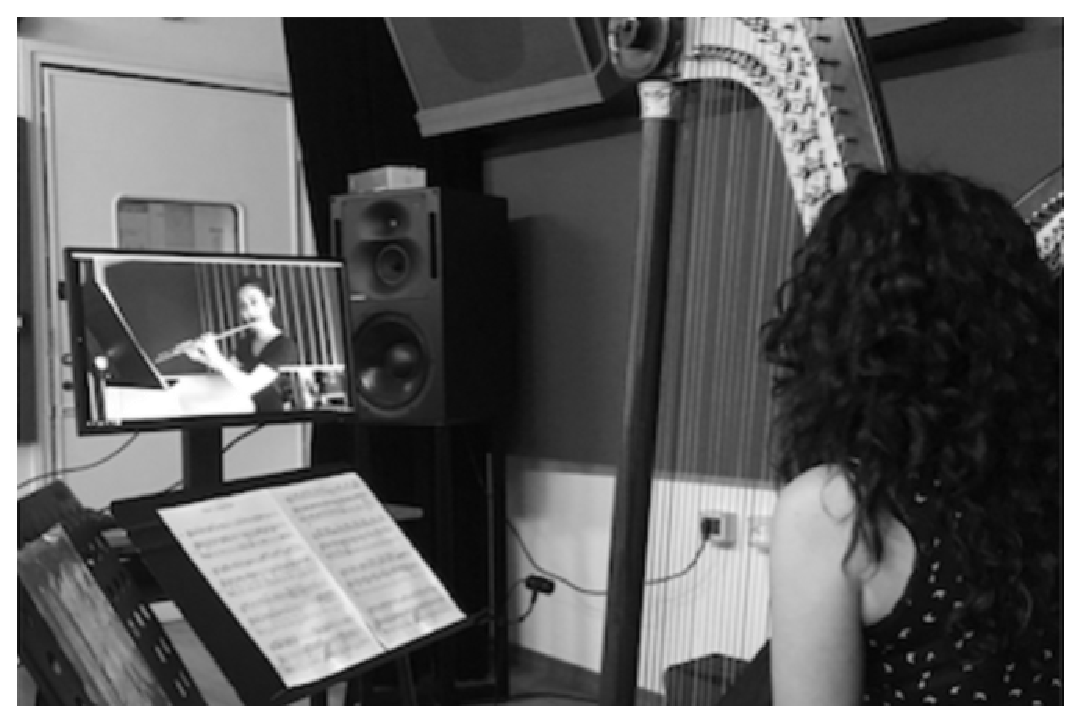
\includegraphics[width=\textwidth]{img/as.eps}
		\caption{View of Room 1}
		\label{subfig:as}
	\end{subfigure}
    \begin{subfigure}[t]{.48\columnwidth}
	\centering        
	%\includegraphics[trim={.5cm 13.7cm 13.5cm .5cm},clip,width=\textwidth]{figures/ann1}
	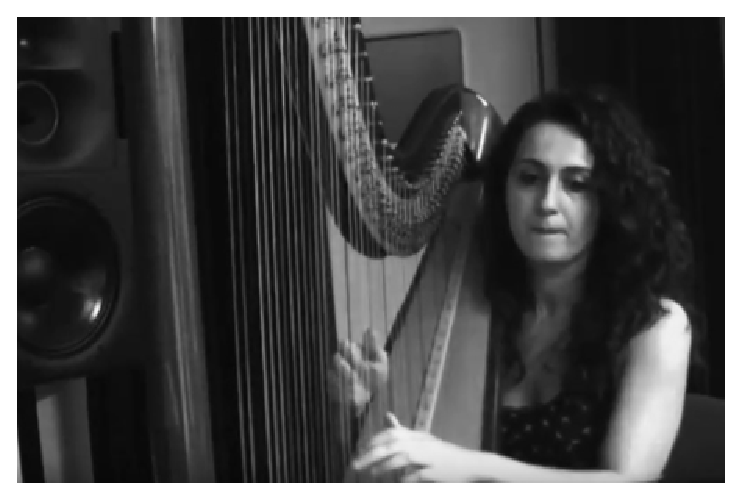
\includegraphics[width=\textwidth]{img/av.eps}
	\caption{View of Musician 1 from Room 2}
	\label{subfig:av}
	\end{subfigure}
    \begin{subfigure}[t]{.48\columnwidth}
	\centering        
	%\includegraphics[trim={.5cm 13.7cm 13.5cm .5cm},clip,width=\textwidth]{figures/ann1}
	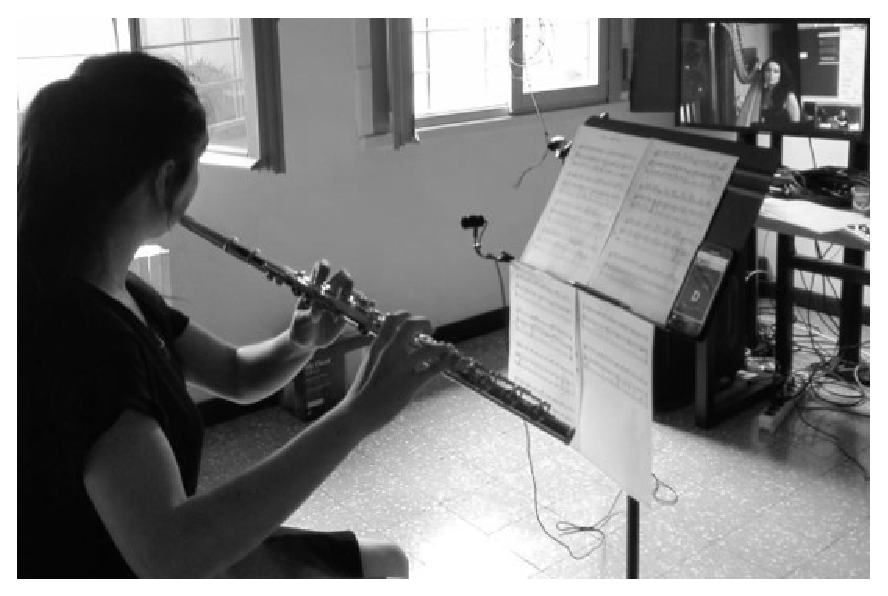
\includegraphics[width=\textwidth]{img/fs.eps}
		\caption{View of Room 2}
	\label{subfig:fs}
	\end{subfigure}
	\begin{subfigure}[t]{.48\columnwidth}
	\centering        
	%\includegraphics[trim={.5cm 13.7cm 13.5cm .5cm},clip,width=\textwidth]{figures/ann1}
	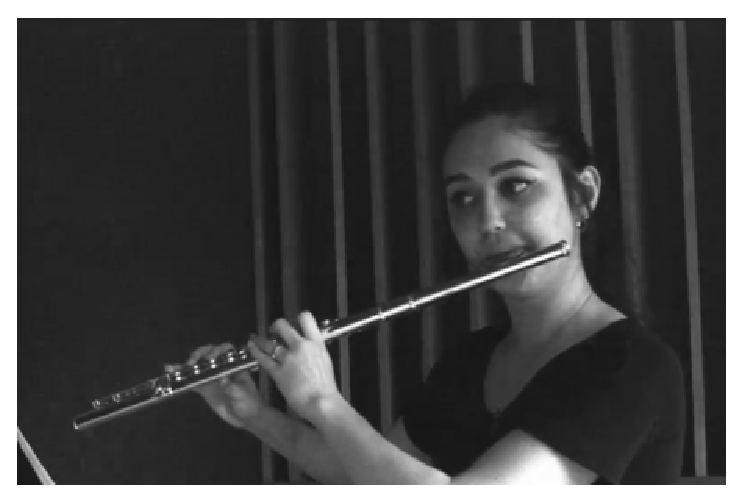
\includegraphics[width=\textwidth]{img/fv.eps}
	\caption{View of Musician 2 from Room 1}
	\label{subfig:fv}
\end{subfigure}

	\quad 
	\caption{View of Rooms 1 and 2 and the corresponding view seen on the screen}\label{fig:afsv}

\end{figure*}


%\section{Results and discussion}\label{sec:discussion}

\subsection{Evaluation}
We could observe different strategies of musical coordination and interpretation, based on breathing signaling and communicative gestures to keep synchronization, especially for attacks and the duration of sustained notes. In this case, the no sight condition deeply affected the expressiveness of the performance. In full visual occlusion, the performers rely mostly on acoustic cues to keep the tempo, with the apparent effect of a rather “gallopping” playing.

Concerning the musical sequences, they reported the more completeness and effectiveness of test 1, while they found the looping sequences quite easy, except for the change of 


The partial occlusion condition somewhat mimics a possible strategy for visual information reduction in remote performance (blob). 


\subsection{Future directions}




\section{Conclusion}\label{sec:conclusion}
%This part presents the key findings in substance. Avoid simple enumeration of the following material. It is desirable to provide a link to existing articles and grants. 

Using Networked Music Performances for pedagogical scenarios require a deep investigation on the topic to find metrics, factors and aspects that may help musicians to improve their musical skills.

In this paper, we presented a framework for conducting perceptual experiments to continue this investigation for the purposes of the project InterMUSIC. We then discussed two experiments conducted using the framework and the preliminary results that we observed.

Starting from this results, we described the areas of investigation that we intend to conduct for the project, with the final goal of developing a platform for NMPs in pedagogical scenarios that also work with general-purpose hardware.

Beyond this areas, in future work we intend to further develop the formalization of the framework into an ontology, which will be integrated in the NMP tools, in order to collect and analyze a number of semantically-annotated rehearsal or lessons \cite{Kolazi2013}. 

 


\section*{Acknowledgment}
%\section{Acknowledgment}
%The work described in this paper is part of the project InterMUSIC, 
This study was conducted for the InterMUSIC project,
which received the financial support of the Erasmus+ National Agency under the KA203 Strategic Partnership action under grant number: 2017-1-IT02-KA203-036770.

The authors would like to thank the participants of the  pilot tests for their effort and their availability to be contacted for further experiments. 

\begin{thebibliography}{6}


\bibitem{Lazzaro2001}
J.Lazzaro and J.Wawrzynek, ``A case for network musical performance'', in \emph{Proc. NOSSDAV Workshop}, Jun. 2001, pp. 157--166. 


\bibitem{IorwerthNMP2015}
M. Iorwerth, D. Moore and D. Knox, ``Challenges of using Networked Music Performance in education'', in  \emph{Proc. AES Conference}, Aug. 2015, pp. 157--166. 


\bibitem{MIDItoolbox}
T. Eerola and P. Toiviainen, \emph{MIDI Toolbox: MATLAB Tools for Music Research}, Finland: University of Jyv{\"a}skyl{\"a},  2004.

\bibitem{Kolazi2013}
\c{S}. Kolozali and M. Barthet and G. Fazekas and M. Sandler, ``Automatic Ontology Generation for Musical Instruments Based on Audio Analysis'', in \emph{IEEE Transactions on Audio, Speech, and Language Processing}, Oct. 2013, pp. {2207--2220}
%	year={2013}, 
%	volume={21}, 
%	number={10}, 

\bibitem{camurri2010visual}
A. Camurri and T. Moeslund, Chap. ``Visual gesture recognition'' in \emph{Musical Gestures: Sound, Movement, and Meaning}, Edited by R. I. God{\o}y, and M. Leman, Routledge, 2010

\bibitem{Canclini2015}
A. Canclini, L. Mucci, F. Antonacci, A. Sarti, S. Tubaro, ``A Methodology for estimating the ratiationpattern of a violin during the performance'' \emph{in Proc. of the European Signal Processing Conference (EUSIPCO)}, 2015

\bibitem{Olmos2009}
A. Olmos, M. Brulé, N. Bouillot, M. Benovoy, J. Blum, H. Sun, N. W. Lund, and J. R. Cooperstock, ``Exploring the role of latency and orchestra placement on the networked performance of a distributed opera'' \emph{in 12th annual international workshop on presence}, 2009

\bibitem{Goto2010}
M. Goto, ``An Audio-based Real-time Beat Tracking System for Music With or Without Drum-sounds'' in \emph{Journal of New Music Research}, 30:2, pp. 159-171, 2010

%30:2, 159-171, DOI: 10.1076/jnmr.30.2.159.7114

\bibitem{conductor2008}
A. Nijholt, D. Reidsma ; R. Ebbers and M. ter Maat, ``The Virtual Conductor: Learning and Teaching about Music, Performing, and Conducting'', in \emph{proc. of the IEEE International Conference on Advanced Learning Technologies}, 2008

\bibitem{duffy2017new}
S. Duffy, and P. Healey, ``A new medium for remote music tuition'', in \emph{Journal of Music, Technology \& Education}, 2017, pp 5--27

\bibitem{uk5G}
UK 5G Innovation Network, Video: World's First 5G Distributed Music Concert, Web: https://uk5g.org/discover/read-articles/video-worlds-first-5g-distributed-music-concert/

%	volume={10},
%	number={1},
%	pages={5--29},
%	year={2017},
%	publisher={Intellect}

%	m
%	\bibitem{Cover}
%	\textit{(Example for books)} T.M.Cover and J.A. Thomas, \emph{Elements of Information Theory}. New York: Wiley, 1991.
%	
%	\bibitem{Dobrushin}
%	\textit{(Example for articles)} R.L. Dobrushin, ``Optimum information transmission through a channel with unknown parameters'',  \emph{Radiotech.Electron.}, vol.4, Dec.1959, pp. 1951-1956.
%	
%	\bibitem{Blachman}
%	\textit{(Example for articles)} N.M. Blachman, ``Communication as a game'', \emph{in Proc. WESCON Conf.}, Aug. 1957, pp. 61-66.
%	
%	\bibitem{IEEE}
%	\textit{(Example for web-links)} IEEE official website, Manuscript Templates for Conference Proceedings, Web: http://www.ieee.org/conferences\_events/conferences/publishing/templates.\newline html.
%	
%	\bibitem{Elissa}
%	\textit{(Example for unpublished references)} K. Elissa, ``Title of paper if known'', unpublished.
%	
%	\bibitem{Nicole}
%	\textit{(Example for references have been accepted for publication)} R. Nicole, ``Title of paper with only first word capitalized'', J. Name Stand. Abbrev., in press.
%	

\bibitem{RottondiOverview}
C.Rottondi, C. Chafe, C. Allocchio, AND A. Sarti
An Overview on Networked Music Performance Technologies, \emph{IEEE Access},4,2016



\bibitem{Lakiotakis}
E. Lakiotakis, C. Liaskos, X. Dimitropoulos, Improving networked music performance systems using application-network collaboration,\emph{Concurrency and Computation: Practice and Experience},Wiley Online Library, 2018

\bibitem{RottondiFeature}
C. Rottondi, M. Buccoli, M. Zanoni, D. Garao,  G. Verticale, A. Sarti,  Feature-Based Analysis of the Effects of Packet Delay on Networked Musical Interactions, \emph{Journal of the Audio Engineering Society}, 63(11), 864-875.



% Chafe clapping experiments
\bibitem{Chafe3}
C. Chafe, J-P. Caceres, M. Gurevich, Effect of temporal separation on synchronization in rhythmic performance,
\emph{Perception}, 39(7): 982-992, 2010

\bibitem{Chafe2}
C. Chafe, M. Gurevich Network Time Delay and Ensemble Accuracy: Effects of Latency, Asymmetry,
\emph{Proc. of the AES 117th Conf.}, SF, 2004

\bibitem{Chafe1}
C. Chafe, M. Gurevich, et al. “Effect of Time Delay on Ensemble Accuracy”
\emph{Proc. 2004 Intl. Soc. Musical Acoustics}, Nara, 2004


% BArbosa

\bibitem{Carot07networkmusic}
Er Car\^ot and Christian Werner,Network music performance - problems, approaches and perspectives,
    \emph{International School of new Media, Institute of Telematics, University of Lübeck. Music in the Global Village - Conference}
    ,2007

\bibitem{Gurevich11}
M. Gurevich, D. Donohoe, S. Bertet, Ambisonic spatialization for networked music performance.


\bibitem{gurevich2011ambisonic}
M. Gurevich, D. Donohoe, S. Bertet,
  Ambisonic Spatialization for Networked Music Performance,
  year={2011},
  \emph{International Community for Auditory Display}, 2011

% reverberation studies
\bibitem{carot2009towards}
 Towards a comprehensive cognitive analysis of delay-influenced rhythmical interaction,
  A. Car{\^o}t, C. Werner and T. Fischinger,
  \emph{ICMC},
  2009

\bibitem{FarnerReverb}
S. Farner, A. Solvang, A. Sæbø and Peter Svensson, Ensemble hand-clapping experiments under
the influence of delay and various acoustic
environments,\emph{Journal of the Audio Engineering Society}, 57(12),
  pp 1028--1041, 2009


% LOLA
\bibitem{drioli2013networked}
C. Drioli, C. Allocchio, and N. Buso,
  Networked performances and natural interaction via LOLA: Low latency high quality A/V streaming system,
  \emph{Information Technologies for Performing Arts, Media Access, and Entertainment}, Springer, 2013
  pp.240--250,


%	
%	\bibitem{Cover}
%	\textit{(Example for books)} T.M.Cover and J.A. Thomas, \emph{Elements of Information Theory}. New York: Wiley, 1991.
%	
%	\bibitem{Dobrushin}
%	\textit{(Example for articles)} R.L. Dobrushin, ``Optimum information transmission through a channel with unknown parameters'',  \emph{Radiotech.Electron.}, vol.4, Dec.1959, pp. 1951-1956.
%	
%	\bibitem{Blachman}
%	\textit{(Example for articles)} N.M. Blachman, ``Communication as a game'', \emph{in Proc. WESCON Conf.}, Aug. 1957, pp. 61-66.
%	
%	\bibitem{IEEE}
%	\textit{(Example for web-links)} IEEE official website, Manuscript Templates for Conference Proceedings, Web: http://www.ieee.org/conferences\_events/conferences/publishing/templates.\newline html.
%	
%	\bibitem{Elissa}
%	\textit{(Example for unpublished references)} K. Elissa, ``Title of paper if known'', unpublished.
%	
%	\bibitem{Nicole}
%	\textit{(Example for references have been accepted for publication)} R. Nicole, ``Title of paper with only first word capitalized'', J. Name Stand. Abbrev., in press.
%	

\end{thebibliography}

\end{document}